\documentclass[11pt]{article}
\usepackage[margin=1in]{geometry}
\usepackage{amsmath,amssymb}
\usepackage{booktabs}
\usepackage{graphicx}
\usepackage[hidelinks]{hyperref}
\usepackage{xcolor}
\usepackage{natbib}
\bibliographystyle{plainnat}

\title{The Action Lags the Answer:\\
An Agent's Tool Commitment Becomes Causally Steerable\\
Deeper Than Its Verbalizable Answer, in Two Architectures}
\author{Caio Vicentino\\
OpenInterpretability \quad \href{https://orcid.org/0009-0003-4331-6259}{ORCID 0009-0003-4331-6259}}
\date{July 2026}

\begin{document}
\maketitle

\begin{abstract}
\citet{anthropic2026workspace} show that language models carry an emergent, verbalizable
\emph{global workspace} (``J-space''): a few dozen concepts, read out by a Jacobian lens, whose
coordinate interventions causally reroute multi-hop \emph{answers} at mid-network depth. Their study
contains no agentic content, leaving open whether an agent's \emph{action} selection is reachable at
the same depth as its verbalizable answer. We test this on \textbf{two} open-weights reasoning
agents---a Qwen3.6-27B (dense) coding agent and gpt-oss-20b (mixture-of-experts)---using a row-restricted J-lens
estimator whose readout directions we validate with a specificity control (a steer flips a held
answer $17/20$ at half the residual norm, while random and unrelated directions flip $0/20$ and an
equal-magnitude random push does not even move the answer). With the instrument validated, we find a
\textbf{robust depth lag}: the agent's tool commitment becomes causally steerable via the verbalizable
direction \emph{strictly deeper} than the verbalizable answer. On Qwen the answer is steerable from
the mid-workspace (L27, 42\% depth; $11/20$ vs random $0$) where the action is not
($0/60$, \emph{worse} than random $21$), the action first steerable at the workspace tail (L47, 73\%,
$60/60$). On gpt-oss the answer's onset is later (the tail, $14/20$ vs random $0$) and the action's
later still (only the motor band, $40/40$ vs random $4$; not the tail, $0/40$). The absolute onset
depths are model-dependent; the lag is invariant---on both models there is a band where the
verbalizable answer is steerable and the action is not (the gpt-oss decision point is a weaker probe,
edit-commit fidelity $0.14$ vs $0.23$, so it corroborates rather than leads). The action's readout also emerges late
(AUROC peaks $0.74$ at L47 in Qwen), and projecting out the top-10 verbalizable directions at the
decision point leaves the commitment differential intact ($0.174 \rightarrow 0.167$). We
\emph{localize} (not discover) the knowledge--action gap \citep{basu2026gap} as this
answer$\rightarrow$action depth lag; the contribution is the lag, its cross-architecture replication,
and the null ablation. Scoped implication: a J-lens-style verbalizable monitor reads a reasoning
agent's answer at a shallower depth---and in a band before---its action commitment. Ledger, vectors,
pre-registration, and a recompute-every-number evaluation are released; the readout curve recomputes
offline to $10^{-6}$ (16/16 layers) and the dissociation numbers reproduce under an independent
re-implementation.
\end{abstract}

\section{Introduction}
A reasoning agent that decides to call an irreversible tool has, somewhere in its forward pass,
committed to that action. Where? \citet{anthropic2026workspace} give a sharp new vocabulary for
``where'': a Jacobian lens (J-lens) reveals an emergent \emph{global workspace}, a small set of
verbalizable concepts occupying a middle band of depth, whose coordinates can be swapped to causally
change a model's multi-hop \emph{answer}. Ablating the top workspace directions destroys multi-hop
reasoning while sparing surface parsing. The paper studies pretrained-style completions; it contains
no agent, tool-use, or action content, leaving whether \emph{action selection or tool routing
bypasses the workspace} an open question for deployed agents.

Our prior arc supplies the exact complementary prior. For a long-horizon coding agent we showed the
control of an action lives not at the mid-layer ``task is done'' verdict but in a late, task-matched
commitment band $\sim$30 layers downstream \citep{vicentino2026lever}, that this late lever brakes
irreversible actions \citep{vicentino2026brake}, and that a reasoning model's chain-of-thought is
causal for its action only in that same late band \citep{vicentino2026late}. In the workspace
vocabulary this predicts a specific, falsifiable claim: the agent's action commitment becomes
reachable by the verbalizable direction \emph{later in depth} than the answer. We test it directly.

\paragraph{Contribution.} On \emph{two} open-weights reasoning agents (a dense 27B and an MoE 20B) we
establish a robust depth lag: the verbalizable-workspace direction that causally reroutes a held
\emph{answer} at some depth does \emph{not} reroute the agent's \emph{tool commitment} at that same
depth (it is at or below a random control there); the action becomes specifically steerable only
strictly deeper. The absolute onset depths differ by model (mid-workspace vs the tail for the answer;
tail vs motor for the action), but on both there is a band where the answer is steerable and the
action is not. Ablating the verbalizable subspace at the decision point does not disturb the
commitment. We are careful about novelty (\S\ref{sec:related}): we neither discover the
knowledge--action gap nor claim action is
merely deeper than the answer---both are known. The new object is the \emph{dissociation plus null
ablation}, and its scoped monitoring implication.

\section{Related work and novelty}\label{sec:related}
A post-result literature scan returns no work testing whether an agent's action commitment routes
through the \emph{emergent} workspace; three neighbors bound our claims and are differentiated here.
\citet{basu2026gap} document a knowledge--action gap---internal probes separate cases the model
fails to act on ($98\%$ vs $45\%$)---but treat it as an actionability limit; we do not claim the gap,
we \emph{localize} it as an answer$\rightarrow$action depth lag and show the mid-workspace direction
that reroutes the answer is not yet reachable through the action there. \citet{when2tool2026} read \emph{whether} a tool
is needed with a linear probe; we study \emph{which} tool is committed and its causal routing, and
show it is dissociated from the workspace direction and survives its ablation. \citet{tooldep2026}
decode tool-call dependency topology from the residual stream while explicitly disclaiming behavioral
control, and \citet{planning2026} show semantic direction forms early while deep layers stabilize
outputs; because tool-related signals are linearly \emph{readable} early, we scope our claim to the
\emph{specific causal steerability of the which-tool commitment via the verbalizable direction}, not
readability in general. Global-workspace models of cognition in networks
\citep{goyal2021gwt,vanrullen2021gwt} \emph{impose} a workspace as an architectural module; we test an
\emph{emergent} one and ask whether action routes through it.

\section{Method}\label{sec:method}
\paragraph{Model and decision points.} Qwen3.6-27B (64 layers; depth\% $= \ell/64$). From 99
SWE-bench Pro trajectories \citep{vicentino2026brake} we take 60 deterministic \texttt{edit}
(\texttt{str\_replace\_editor}) and 60 \texttt{bash} decision points, prefill-only, following the
protocol of \citet{vicentino2026lever}. Answers are a constructed 20-item few-shot two-hop QA set
(single-token answers; $20/20$ baseline accuracy).

\paragraph{Row-restricted J-lens estimator.} For a single-token concept $v$ and layer $\ell$ we
estimate the readout row $g_{v,\ell} = \partial\,\mathrm{logit}_v(\text{final position})/\partial
h_{\ell,\text{final}}$ by one backward pass per $(v,\text{prompt})$, parameters frozen and the
embedding made the sole gradient leaf, averaged over an on-distribution estimation set. This is the
diagonal (same-position) readout direction, not the full Jacobian matrix; we do not claim a complete
reproduction of the J-lens.

\paragraph{Instrument validation (specificity control).} The pre-registered coordinate \emph{swap}
$h \leftarrow h + V(\sigma(c)-c)$ is a near-no-op in this basis (the raw-gradient projections are
near-equal, $c_{\text{correct}}\approx c_{\text{alt}}$), so we validate and use a \emph{steer} along
the normalized $(g_{\text{alt}}-g_{\text{correct}})$ direction scaled to $\alpha\lVert h\rVert$---a
disclosed deviation to a second Anthropic-used intervention on the same directions. Table
\ref{tab:spec} shows the steer is specific: at $\alpha{=}0.5$ it flips a held answer to the designated
alternative $17/20$, while unrelated-pair and random directions flip $0/20$ and a random push of
equal magnitude does not move the answer at all. (A readout-correlation check is uninformative here:
RMSNorm is degree-0 homogeneous, so by Euler's theorem $g_v\!\cdot h \approx 0$ by construction.)

\begin{table}[h]\centering\small
\begin{tabular}{lcccc}
\toprule
$\alpha$ & contrast$\rightarrow$alt & unrelated$\rightarrow$alt & random$\rightarrow$alt & random moved off correct \\
\midrule
0.5 & \textbf{17/20} & 0/20 & 0/20 & 0/20 \\
1.0 & \textbf{20/20} & 0/20 & 0/20 & 19/20 \\
\bottomrule
\end{tabular}
\caption{Specificity control: the estimated readout direction is causal and specific; equal-magnitude
random pushes do not reroute (and at $\alpha{=}0.5$ do not even move) the answer.}
\label{tab:spec}
\end{table}

\section{Results}
\paragraph{H1: the action is readable only in the workspace tail.}
Figure~\ref{fig:h1} plots the AUROC of $(g_{\text{edit}}-g_{\text{bash}})\!\cdot h$ separating edit-
from bash-decision points by depth. It is near chance through most of mid-workspace, first exceeding
chance only near L35, and rises to a peak of $0.74$ at layer 47 (73\%), sustaining $0.59$--$0.69$ into
the motor band. The action's verbalizable readout emerges at the workspace tail, not mid-workspace.
(The curve recomputes offline from the
public vectors and residuals to $10^{-6}$ at all 16 layers.)

\paragraph{H2 and the dissociation: answers reroute in mid-workspace; the action does not.}
We steer the commitment along $(g_{\text{other}}-g_{\text{taken}})$ at the decision points
($\alpha{=}0.5$), band-wise, against a random-direction control, and---parallel and apples-to-apples
---steer the \emph{answer} per band (Figure~\ref{fig:dissoc}, Table~\ref{tab:dissoc}). At mid-workspace
the verbalizable direction \emph{specifically} reroutes answers ($11/20$ vs random $0$) but the action
steer is \emph{worse than random} ($0/60$ vs $21/60$): no specific workspace-mediated rerouting of the
commitment. Specific action control appears at the tail ($60/60$ vs random $23$) and completes at motor---so the
action is not absent from the workspace, it is reachable only from the workspace \emph{tail} onward,
strictly deeper than the answer. Because the identical magnitude at the identical layers reroutes the
answer but not the action, the mid-workspace action result is not a magnitude/disruption artifact.
Decoding the mid-workspace action steer confirms this: the global argmax is dominated by structural
tokens (\texttt{>} 47/60, newline 8/60; only 1/60 a tool token, 6 distinct tokens), i.e.\ the
mid-workspace intervention perturbs emission without producing a clean committed tool call.

\begin{table}[h]\centering\small
\begin{tabular}{lcc}
\toprule
band & answer: contrast$\rightarrow$alt (random) & action: edit$\rightarrow$bash (random) \\
\midrule
mid-workspace (L27--43) & \textbf{11/20 (0)} & \textbf{0/60 (21)} \\
tail (L47--55)          & 20/20 (0) & 60/60 (23) \\
motor (L59--63)         & 20/20 (0) & 60/60 (21) \\
\bottomrule
\end{tabular}
\caption{The dissociation. Same steer, same magnitude, same layers: the verbalizable direction
reroutes the answer in mid-workspace but not the action.}
\label{tab:dissoc}
\end{table}

\paragraph{H3: the commitment survives ablation of the verbalizable subspace.}
Projecting out the top-10 verbalizable directions (by lens activation on the agent distribution) at
the decision points leaves the task-appropriate commitment differential essentially unchanged:
$P(\text{edit})$ at edit points $0.474\rightarrow0.473$, at bash points $0.299\rightarrow0.306$;
differential $0.174\rightarrow0.167$ (from unrounded values; Figure~\ref{fig:abl}). The commitment does not live in the
verbalizable subspace at the decision position---the load-bearing rebuttal to ``you are re-reading an
early-decodable tool signal.''

\paragraph{Cross-model: the lag replicates on an MoE architecture.}
We repeat the instrument validation and the band-wise steer on gpt-oss-20b (24 layers, MoE), with
real decision points reconstructed from the same trajectories in a generic tool-choice format and
bands mapped by depth-percentage (Table~\ref{tab:xmodel}). The specificity control holds (few-shot
two-hop baseline $14/20$; answer flips $20/20$ at motor vs random $1$). The depth lag replicates: at
the tail the verbalizable direction reroutes the answer ($14/20$ vs random $0$) but not the action
($0/40$ vs random $0$), and the action becomes specifically steerable only at the motor band ($40/40$
vs random $4$). The absolute onsets shift---on gpt-oss the answer consolidates later (tail, not
mid-workspace) and the action later still (motor, not tail)---but the invariant is the same
(Figure~\ref{fig:xmodel}): a band where the answer is steerable and the action is not, with the action
strictly deeper. gpt-oss's
generic-format decision points have weaker edit-commitment fidelity (edit-points $P(\text{edit}){=}0.14$
vs bash-points $0.23$); the random-controlled steer specificity is nonetheless clean.

\begin{table}[h]\centering\small
\begin{tabular}{llcc}
\toprule
model & band & answer $\rightarrow$alt (rand) & action edit$\rightarrow$bash (rand) \\
\midrule
Qwen3.6-27B    & mid   & \textbf{11/20 (0)} & \textbf{0/60 (21)} \\
(dense, 64L)   & tail  & 20/20 (0) & 60/60 (23) \\
               & motor & 20/20 (0) & 60/60 (21) \\
\midrule
gpt-oss-20b    & mid   & 1/20 (3)  & 0/40 (9) \\
(MoE, 24L)     & tail  & \textbf{14/20 (0)} & \textbf{0/40 (0)} \\
               & motor & 20/20 (1) & 40/40 (4) \\
\bottomrule
\end{tabular}
\caption{The lag is cross-architecture. Bold marks each model's dissociation band---answer steerable,
action not. The band's absolute depth is model-dependent (mid on Qwen, tail on gpt-oss); on both the
action's steerability onset is strictly deeper than the answer's.}
\label{tab:xmodel}
\end{table}

\begin{figure}[t]\centering
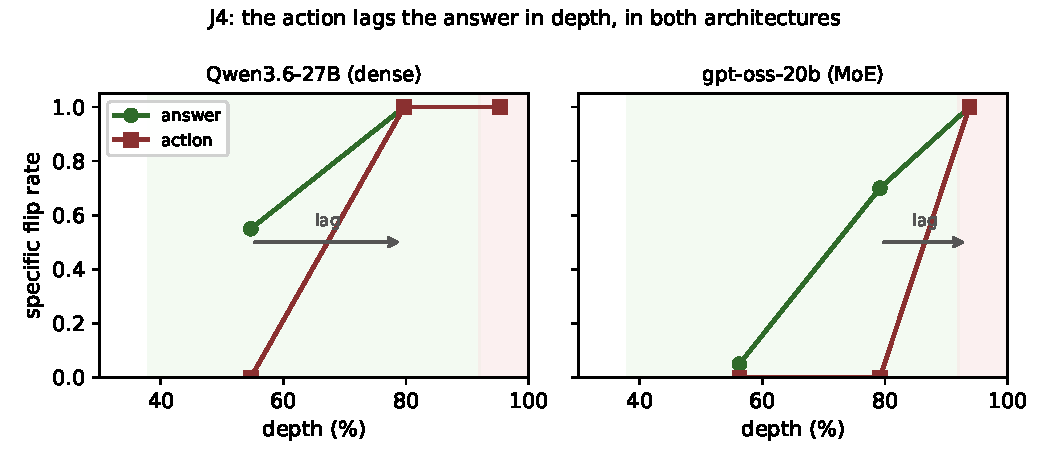
\includegraphics[width=\linewidth]{figures/figJ4_depthlag_xmodel.pdf}
\caption{The reframe headline. In both architectures the verbalizable direction reroutes the
\emph{answer} at a shallower depth than it can reroute the \emph{action} (green before red); the
absolute band shifts with the model but the answer$\rightarrow$action depth lag does not.}
\label{fig:xmodel}
\end{figure}

\begin{figure}[t]\centering
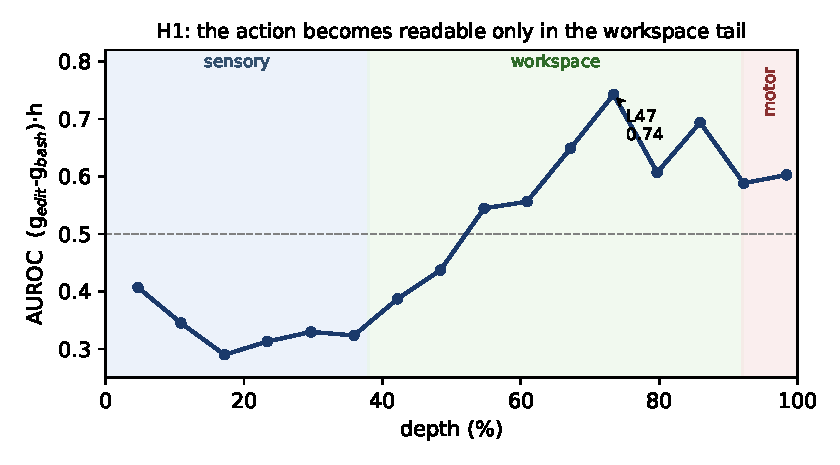
\includegraphics[width=0.86\linewidth]{figures/figJ1_readout_depth.pdf}
\caption{H1. The action's verbalizable readout (AUROC by depth) is near chance through most of mid-workspace and
peaks at the tail (L47, 73\%). Regimes after \citet{anthropic2026workspace}.}
\label{fig:h1}
\end{figure}

\begin{figure}[t]\centering
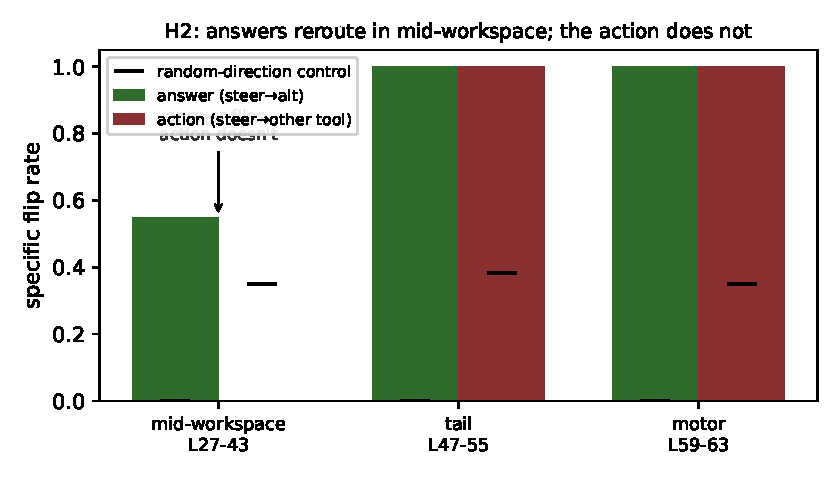
\includegraphics[width=0.86\linewidth]{figures/figJ2_dissociation.pdf}
\caption{H2 dissociation. The verbalizable steer reroutes the \emph{answer} in mid-workspace
($11/20$) but not the \emph{action} ($0/60$, below the random control); both converge at the
tail/motor. Black ticks: random-direction controls.}
\label{fig:dissoc}
\end{figure}

\begin{figure}[t]\centering
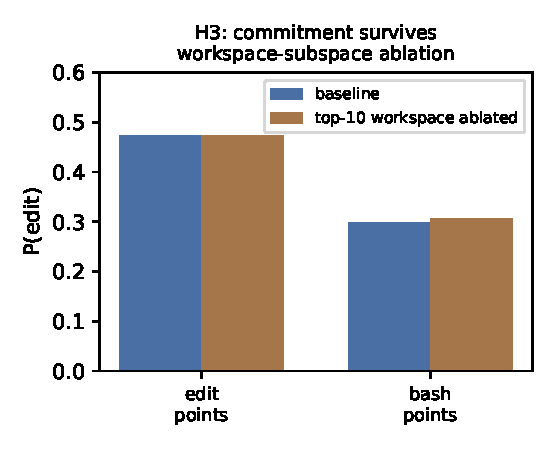
\includegraphics[width=0.52\linewidth]{figures/figJ3_ablation.pdf}
\caption{H3. Ablating the top-10 verbalizable directions at the decision point leaves the
commitment differential intact.}
\label{fig:abl}
\end{figure}

\section{Discussion}
Across a dense 27B and an MoE 20B, the verbalizable direction that \citet{anthropic2026workspace}
steer to change an answer reaches the agent's action commitment \emph{strictly later in depth} than
it reaches the answer: there is a depth band where the held answer is causally steerable and the tool
the agent commits to is not, and the commitment survives ablation of the verbalizable subspace at the
decision point. This localizes the knowledge--action gap \citep{basu2026gap} as an
answer$\rightarrow$action \emph{depth lag} and gives the arc's ``lever is late''
\citep{vicentino2026lever,vicentino2026late} a reading in workspace terms.

\paragraph{Why the action lags (mechanism).} Our prior circuit analysis of this agent
\citep{vicentino2026brake} identifies the commit as written by a small set of late attention heads
(layer 59) that behave as induction/copy heads, promoting the tool-name token by copying it from the
tool-call history rather than composing it from mid-network concepts. Such a late copy operation is
inherently a ``motor'' computation, downstream of and orthogonal to the mid-network concept broadcast
that the verbalizable workspace steers---which is consistent with the lag we observe and with the
commitment surviving ablation of the verbalizable subspace. A full head-level test is left to future
work: prior analysis found layer-59 attention to be output-gated, so cleanly reconstructing per-head
write directions there is nontrivial.

\paragraph{Monitoring implication (scoped).} A J-lens-style verbalizable monitor reads a reasoning
agent's answer/reasoning at a shallower depth---and in a band before---its action commitment: it
would surface the model's stated intent while the committed act is still being decided deeper. This
is scoped to verbalizable (J-lens) monitors on these two open-weights models; we make no
architecture-general claim.

\section{Limitations}
Two open-weights models (a dense 27B and an MoE 20B), one behavior family (edit vs bash), $n{=}60$
action / $20$ answer points on the primary model, prefill-only, single magnitude $\alpha{=}0.5$
(controlled within each band by the random baseline). The depth lag replicates in both models but the
\emph{absolute} onset depths are model-dependent: on the dense model the answer becomes steerable at
mid-network and the action only at the tail, whereas on the MoE model both shift deeper (answer at the
tail, action at the motor band), so we frame the invariant as depth-relative, not as a fixed
``mid-workspace'' band. On the MoE model the synthetic decision point is a weaker probe of the
commit---baseline edit-commit fidelity $0.14$ vs.\ bash $0.23$---so its dissociation is corroborating
rather than primary. The estimator is the row-restricted diagonal, not the full J-lens matrix, and we
use a steer in place of the pre-registered coordinate swap (disclosed; the swap is a near-no-op in
this basis; both are Anthropic-used and the steer is specificity-validated). Tool-related signals are
linearly readable earlier than the commit depth in general
\citep{tooldep2026,when2tool2026}; our claim is about specific causal steerability of the commitment
via the verbalizable direction, not readability. No claim of architecture-generality beyond these two
models; the workspace paper's own agent generality is untested.

\section{Reproducibility}
Public HF ledgers (\texttt{results/jspace\_action.json} for the dense model,
\texttt{results/jspace\_xmodel\_gpt-oss-20b.json} for the MoE), estimated vectors, and decision-point
residuals; harnesses \texttt{scripts/jspace\_action.py}, \texttt{scripts/jspace\_xmodel.py} and
pre-registration released. The evaluation \texttt{scripts/eval\_jspace.py} recomputes the H1 readout
offline from the public vectors and residuals (16/16 layers to $10^{-6}$) and audits the dissociation
logic for both models. Steer and ablation numbers are model-dependent and were verified present in the
public ledgers step-by-step.

\small
\begin{thebibliography}{99}
\bibitem[Anthropic Interpretability Team(2026)]{anthropic2026workspace} Anthropic Interpretability
Team. Verbalizable Representations Form a Global Workspace in Language Models. \emph{Transformer
Circuits Thread}, 2026. transformer-circuits.pub/2026/workspace.
\bibitem[Basu et al.(2026)]{basu2026gap} S.~Basu et al. Interpretability Without Actionability:
Mechanistic Methods Cannot Correct Language Model Errors Despite Near-Perfect Internal
Representations. \emph{arXiv:2603.18353}, 2026.
\bibitem[Sun et al.(2026)]{when2tool2026} C.-E.~Sun, L.~Liu, G.~Yan, Z.~Wang, T.-W.~Weng. LLM Agents
Already Know When to Call Tools --- Even Without Reasoning. \emph{arXiv:2605.09252}, 2026.
\bibitem[Sun \& Kazakov(2026)]{tooldep2026} T.~Sun and D.~Kazakov. Tool-Call Dependency Structure is
Linearly Decodable in LLM Agent Residual Streams. \emph{arXiv:2605.25310}, 2026.
\bibitem[Cui \& Luo(2026)]{planning2026} Z.~Cui and X.~Luo. Do Agents Think Deeper? A Mechanistic
Investigation of Layer-Wise Dynamics in Sequential Planning. \emph{arXiv:2605.27935}, 2026.
\bibitem[Goyal et al.(2021)]{goyal2021gwt} A.~Goyal et al. Coordination Among Neural Modules Through a
Shared Global Workspace. \emph{arXiv:2103.01197}, 2021.
\bibitem[VanRullen \& Kanai(2021)]{vanrullen2021gwt} R.~VanRullen and R.~Kanai. Deep Learning and the
Global Workspace Theory. \emph{Trends in Neurosciences}, 2021. arXiv:2012.10390.
\bibitem[Vicentino(2026a)]{vicentino2026lever} C.~Vicentino. The Lever Is Late: the Knowledge--Action
Gap Is a Layer Gap. \emph{Zenodo}, 2026. DOI 10.5281/zenodo.20534219.
\bibitem[Vicentino(2026b)]{vicentino2026brake} C.~Vicentino. The Commitment Lever Generalizes --- and
It Brakes. \emph{Zenodo}, 2026. DOI 10.5281/zenodo.20679287.
\bibitem[Vicentino(2026c)]{vicentino2026late} C.~Vicentino. The Late Channel: Chain-of-Thought Is
Causal Only When It Changes the Outcome. \emph{Zenodo}, 2026. DOI 10.5281/zenodo.20752895.
\end{thebibliography}

\end{document}
